\documentclass[conference]{IEEEtran}

% ========= パッケージ(順序重要:cite系→他→hyperref最後) =========
\usepackage{cite}
\usepackage{amsmath,amssymb}
\usepackage{siunitx}
\usepackage{graphicx}
\usepackage[caption=false,font=footnotesize]{subfig} % IEEEtran互換
\usepackage{booktabs}
\usepackage{tikz}
\usetikzlibrary{positioning,arrows.meta}
\usepackage{newtxtext,newtxmath}                     % Times系フォント
\usepackage[hidelinks]{hyperref}                     % \texorpdfstring等

% ========= 記号・単位マクロ =========
\newcommand{\Vth}{V_{\mathrm{th}}}
\newcommand{\Ea}{E_{\mathrm{a}}}
\newcommand{\betaW}{\beta} % Weibull slope
\newcommand{\etaW}{\eta}   % Weibull scale
\sisetup{detect-all, per-mode=symbol, separate-uncertainty = true}

% ========= 体裁・間隔(少しだけ詰める) =========
\setlength{\textfloatsep}{9pt plus 2pt minus 2pt}
\setlength{\floatsep}{7pt plus 2pt minus 2pt}
\setlength{\intextsep}{6pt plus 2pt minus 2pt}
\setlength{\abovecaptionskip}{3pt}
\clubpenalty=10000
\widowpenalty=10000

% ========= 図の標準幅(統一調整) =========
\newcommand{\figw}{0.90\linewidth}

% ========= タイトル・著者 =========
\begin{document}

\title{Low-Cost Integration of 1.8-V FeFET on 0.18-$\mu$m CMOS:\\
+1 Mask and a Single ALD Tool, with Reliability Assessment}

\author{\IEEEauthorblockN{Shinichi Samizo}
\IEEEauthorblockA{Independent Semiconductor Researcher\\
Former Engineer at Seiko Epson Corporation\\
Email: shin3t72@gmail.com\quad GitHub: \url{https://github.com/Samizo-AITL}}
}

\maketitle

% ========= Abstract =========
\begin{abstract}
Ferroelectric FETs (FeFETs) are promising CMOS-compatible embedded nonvolatile memories.
This paper demonstrates a 1.8~V FeFET module integrated on a legacy 0.18~$\mu$m CMOS process with only one additional mask and a single ALD tool.
Fabricated devices show endurance exceeding $10^5$ program/erase cycles and retention longer than 10 years at 85$^\circ$C.
Reliability was characterized on FeCAP/FeFET structures: time-zero dielectric breakdown (TZDB), time-dependent dielectric breakdown (TDDB), endurance, and retention.
The approach provides a cost-effective path to extend mature-node lifetimes and to enable embedded NVM for automotive/industrial/IoT, while high-temperature retention remains the key limiter.
\end{abstract}

% ========= Introduction =========
\section{Introduction}
Ferroelectric HfO$_2$-based memories attract attention as CMOS-compatible NVMs~\cite{boscke2011,mueller2012,mikolajick2019,mueller2015}.
While many works target advanced nodes, mature nodes (e.g., 0.18~$\mu$m) remain workhorses in automotive/industrial sectors for cost and longevity.
\textbf{This work contributes}: (i) a +1 mask low-cost module, (ii) only one ALD tool added to the line, (iii) a yield-friendly \textit{SRAM+FeFET} system usage model, and (iv) comprehensive reliability evidence (TZDB, TDDB, endurance, retention) on FeCAP/FeFET.

% ========= Process Integration =========
\section{Process Integration}
Baseline is a 0.18~$\mu$m CMOS platform (1.8~V core, optional 3.3~V I/O).
The FeFET module is inserted after poly definition and salicide/RTA, requiring minimal line modification.

\subsection{Process Flow}
\begin{figure}[!t]
  \centering
  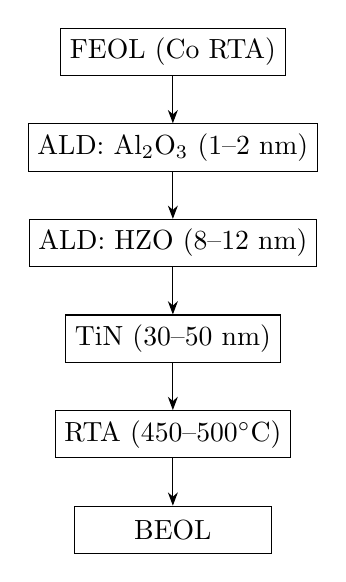
\begin{tikzpicture}[node distance=6mm, every node/.style={draw,rectangle,minimum width=25mm,minimum height=6mm},>=Stealth]
    \node (a) {FEOL (Co RTA)};
    \node (b) [below=of a] {ALD: Al$_2$O$_3$ (1--2 nm)};
    \node (c) [below=of b] {ALD: HZO (8--12 nm)};
    \node (d) [below=of c] {TiN (30--50 nm)};
    \node (e) [below=of d] {RTA (450--500$^\circ$C)};
    \node (f) [below=of e] {BEOL};
    \draw[->] (a) -- (b);
    \draw[->] (b) -- (c);
    \draw[->] (c) -- (d);
    \draw[->] (d) -- (e);
    \draw[->] (e) -- (f);
  \end{tikzpicture}
  \caption{Process flow of FeFET integration.}
  \label{fig:flow}
\end{figure}

\subsection{Cross Section}
\begin{figure}[!t]
  \centering
  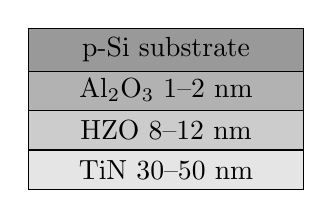
\begin{tikzpicture}
    \node[draw,fill=gray!20,minimum width=35mm,minimum height=5mm,anchor=south west] (tin) at (0,0) {TiN 30--50 nm};
    \node[draw,fill=gray!40,minimum width=35mm,minimum height=5mm,anchor=south west] (hzo) at (0,0.5) {HZO 8--12 nm};
    \node[draw,fill=gray!60,minimum width=35mm,minimum height=5mm,anchor=south west] (al) at (0,1.0) {Al$_2$O$_3$ 1--2 nm};
    \node[draw,fill=gray!80,minimum width=35mm,minimum height=5mm,anchor=south west] (si) at (0,1.5) {p-Si substrate};
  \end{tikzpicture}
  \caption{Cross section of HZO/Al$_2$O$_3$/TiN stack.}
  \label{fig:stack}
\end{figure}

% ========= Devices and Methods =========
\section{Devices and Methods}
Test structures include FeCAPs (flat/comb) and $100~\mu\mathrm{m}\times100~\mu\mathrm{m}$ FeFET cells.
Programming used $\pm$2.3--2.7~V, 1--50~$\mu$s pulses.
A Keysight B1500A with a manual probe station was used.

\textbf{Protocols}: 
TZDB: DC ramp $\approx 0.1$~V/s at RT--125$^\circ$C.
TDDB: constant-voltage stress at $\pm$2.3/2.5/2.7~V, 85$^\circ$C and 125$^\circ$C; Weibull fitting.
Endurance: $\pm$2.5~V, 10~$\mu$s, 10~kHz up to $10^5$ cycles.
Retention: 25$^\circ$C, 85$^\circ$C, 125$^\circ$C with Arrhenius extrapolation.

\begin{table}[!t]
  \centering
  \caption{Reliability test matrix (devices: FeCAP/FeFET).}
  \label{tab:test-matrix}
  \begin{tabular}{@{}ll@{}}
    \toprule
    \textbf{Item} & \textbf{Conditions} \\
    \midrule
    TZDB     & DC ramp $\approx 0.1$ V/s,\ RT--\SI{125}{\celsius} \\
    TDDB     & $\pm$2.3/2.5/2.7 V,\ \SI{85}{\celsius}, \SI{125}{\celsius} \\
    Endurance& $\pm$2.5 V,\ \SI{10}{\micro\second},\ \SI{10}{\kilo\hertz}, up to $10^5$ \\
    Retention& \SI{25}{\celsius}, \SI{85}{\celsius}, \SI{125}{\celsius} \\
    \bottomrule
  \end{tabular}
\end{table}

% ========= Results (Reliability) =========
\section{Results: Reliability}
To keep readability high and figure sizes uniform, the reliability results are split across multiple figures (all with identical width).

\subsection{Time-Zero Dielectric Breakdown (TZDB)}
\begin{figure}[!t]
  \centering
  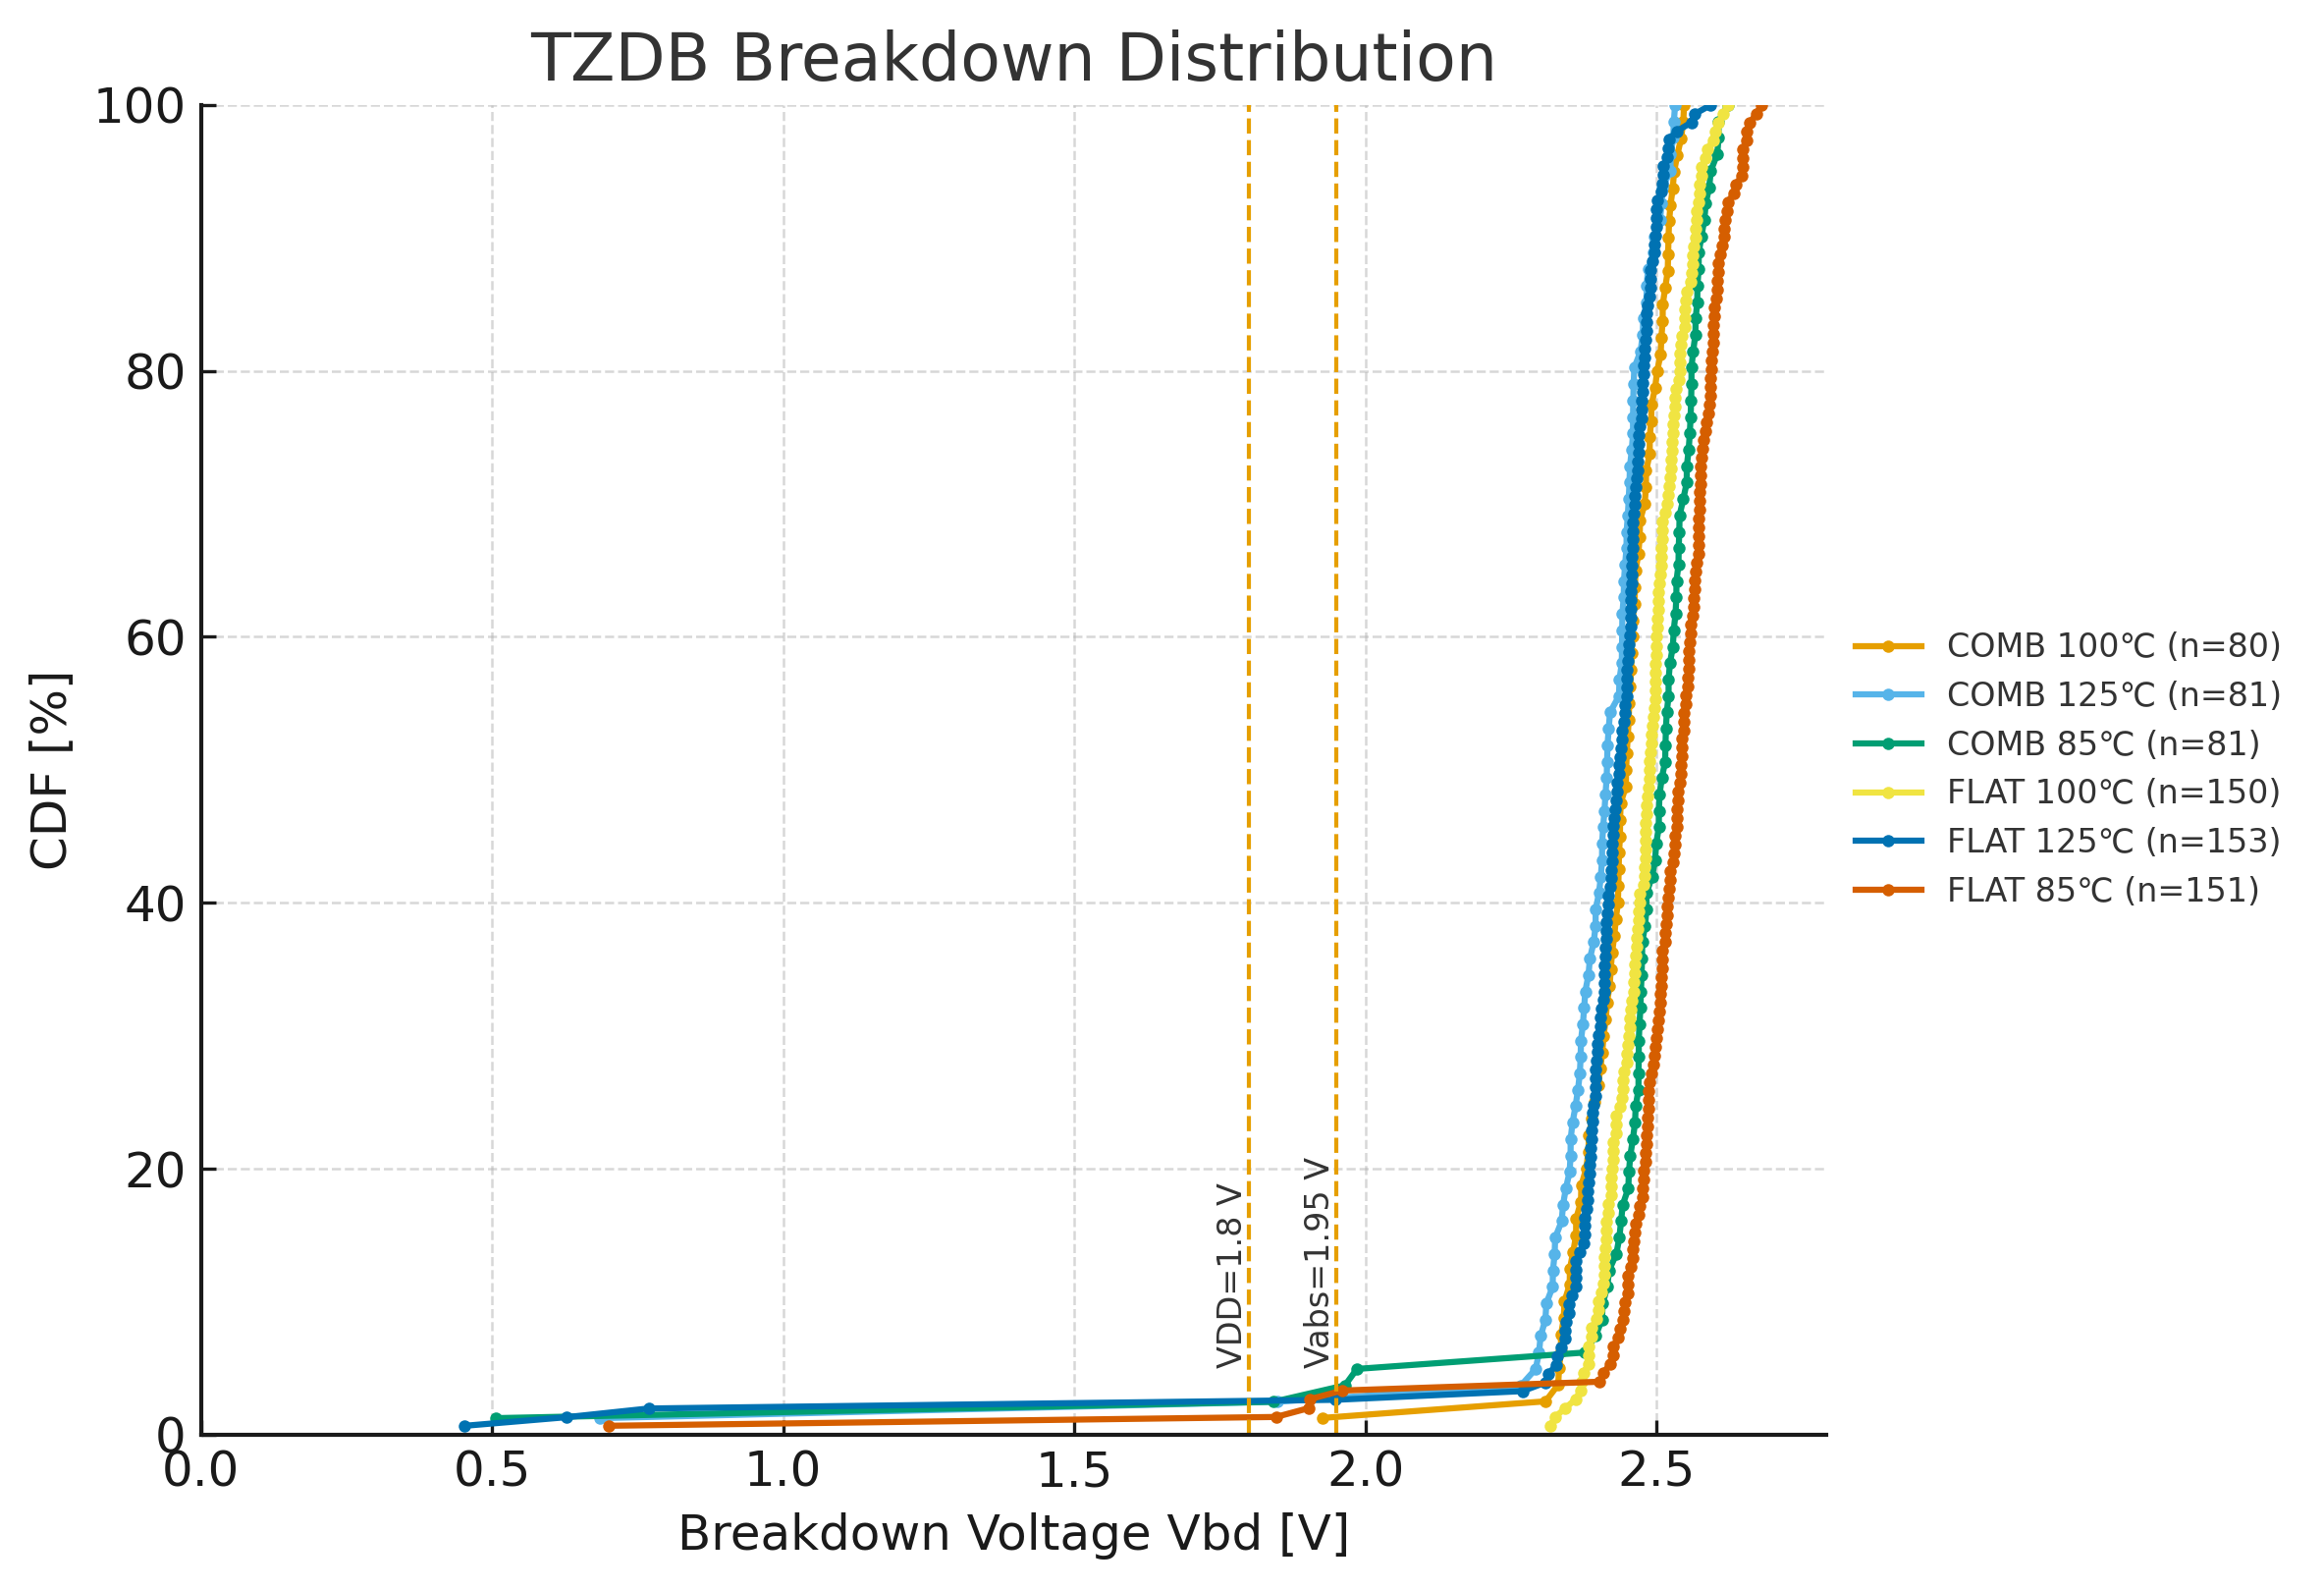
\includegraphics[width=\figw]{figures/fig3_tzdb.png}
  \caption{TZDB distributions of FeCAPs. Early-failure tails imply defect-driven breakdown paths.}
  \label{fig:tzdb}
\end{figure}

\subsection{TDDB under Constant-Voltage Stress}
\begin{figure}[!t]
  \centering
  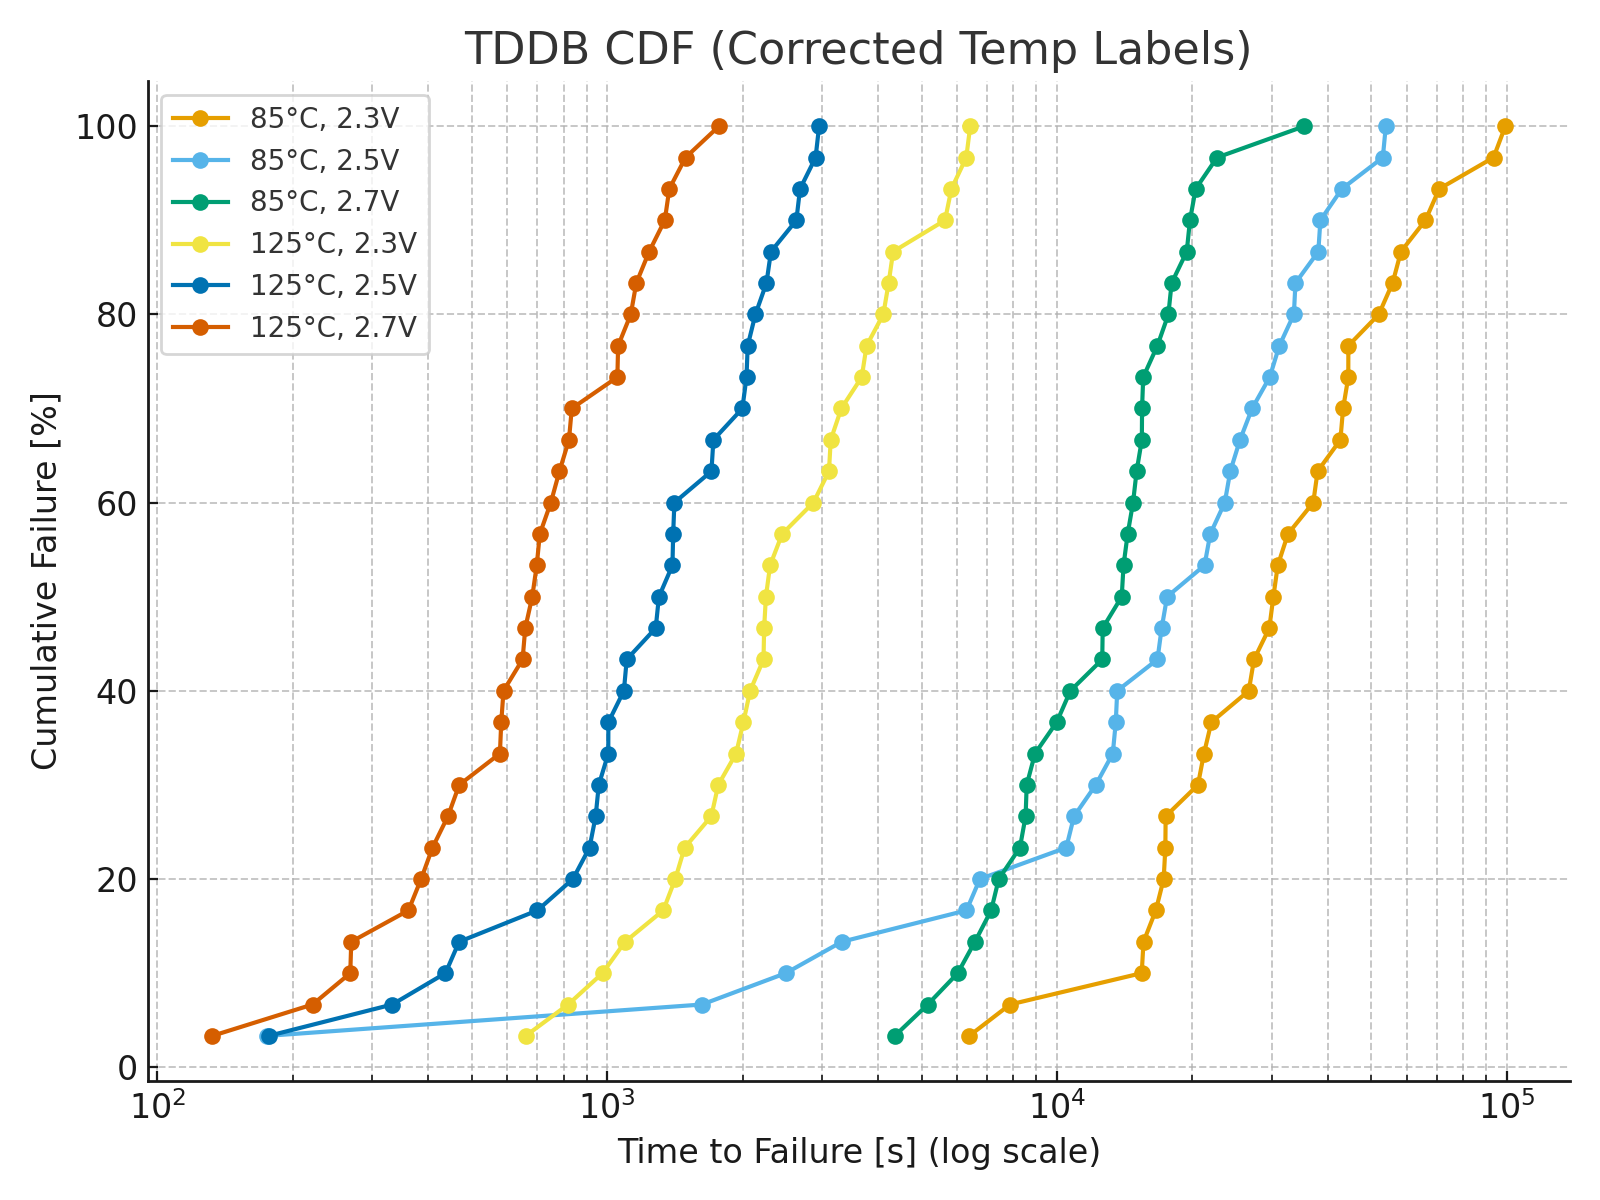
\includegraphics[width=\figw]{figures/fig4_tddb_cdf.png}
  \caption{TDDB cumulative failure probability (CDF) under multiple stress conditions (85$^\circ$C / 125$^\circ$C, $\pm$2.3/2.5/2.7~V).}
  \label{fig:tddb_cdf}
\end{figure}

\begin{figure}[!t]
  \centering
  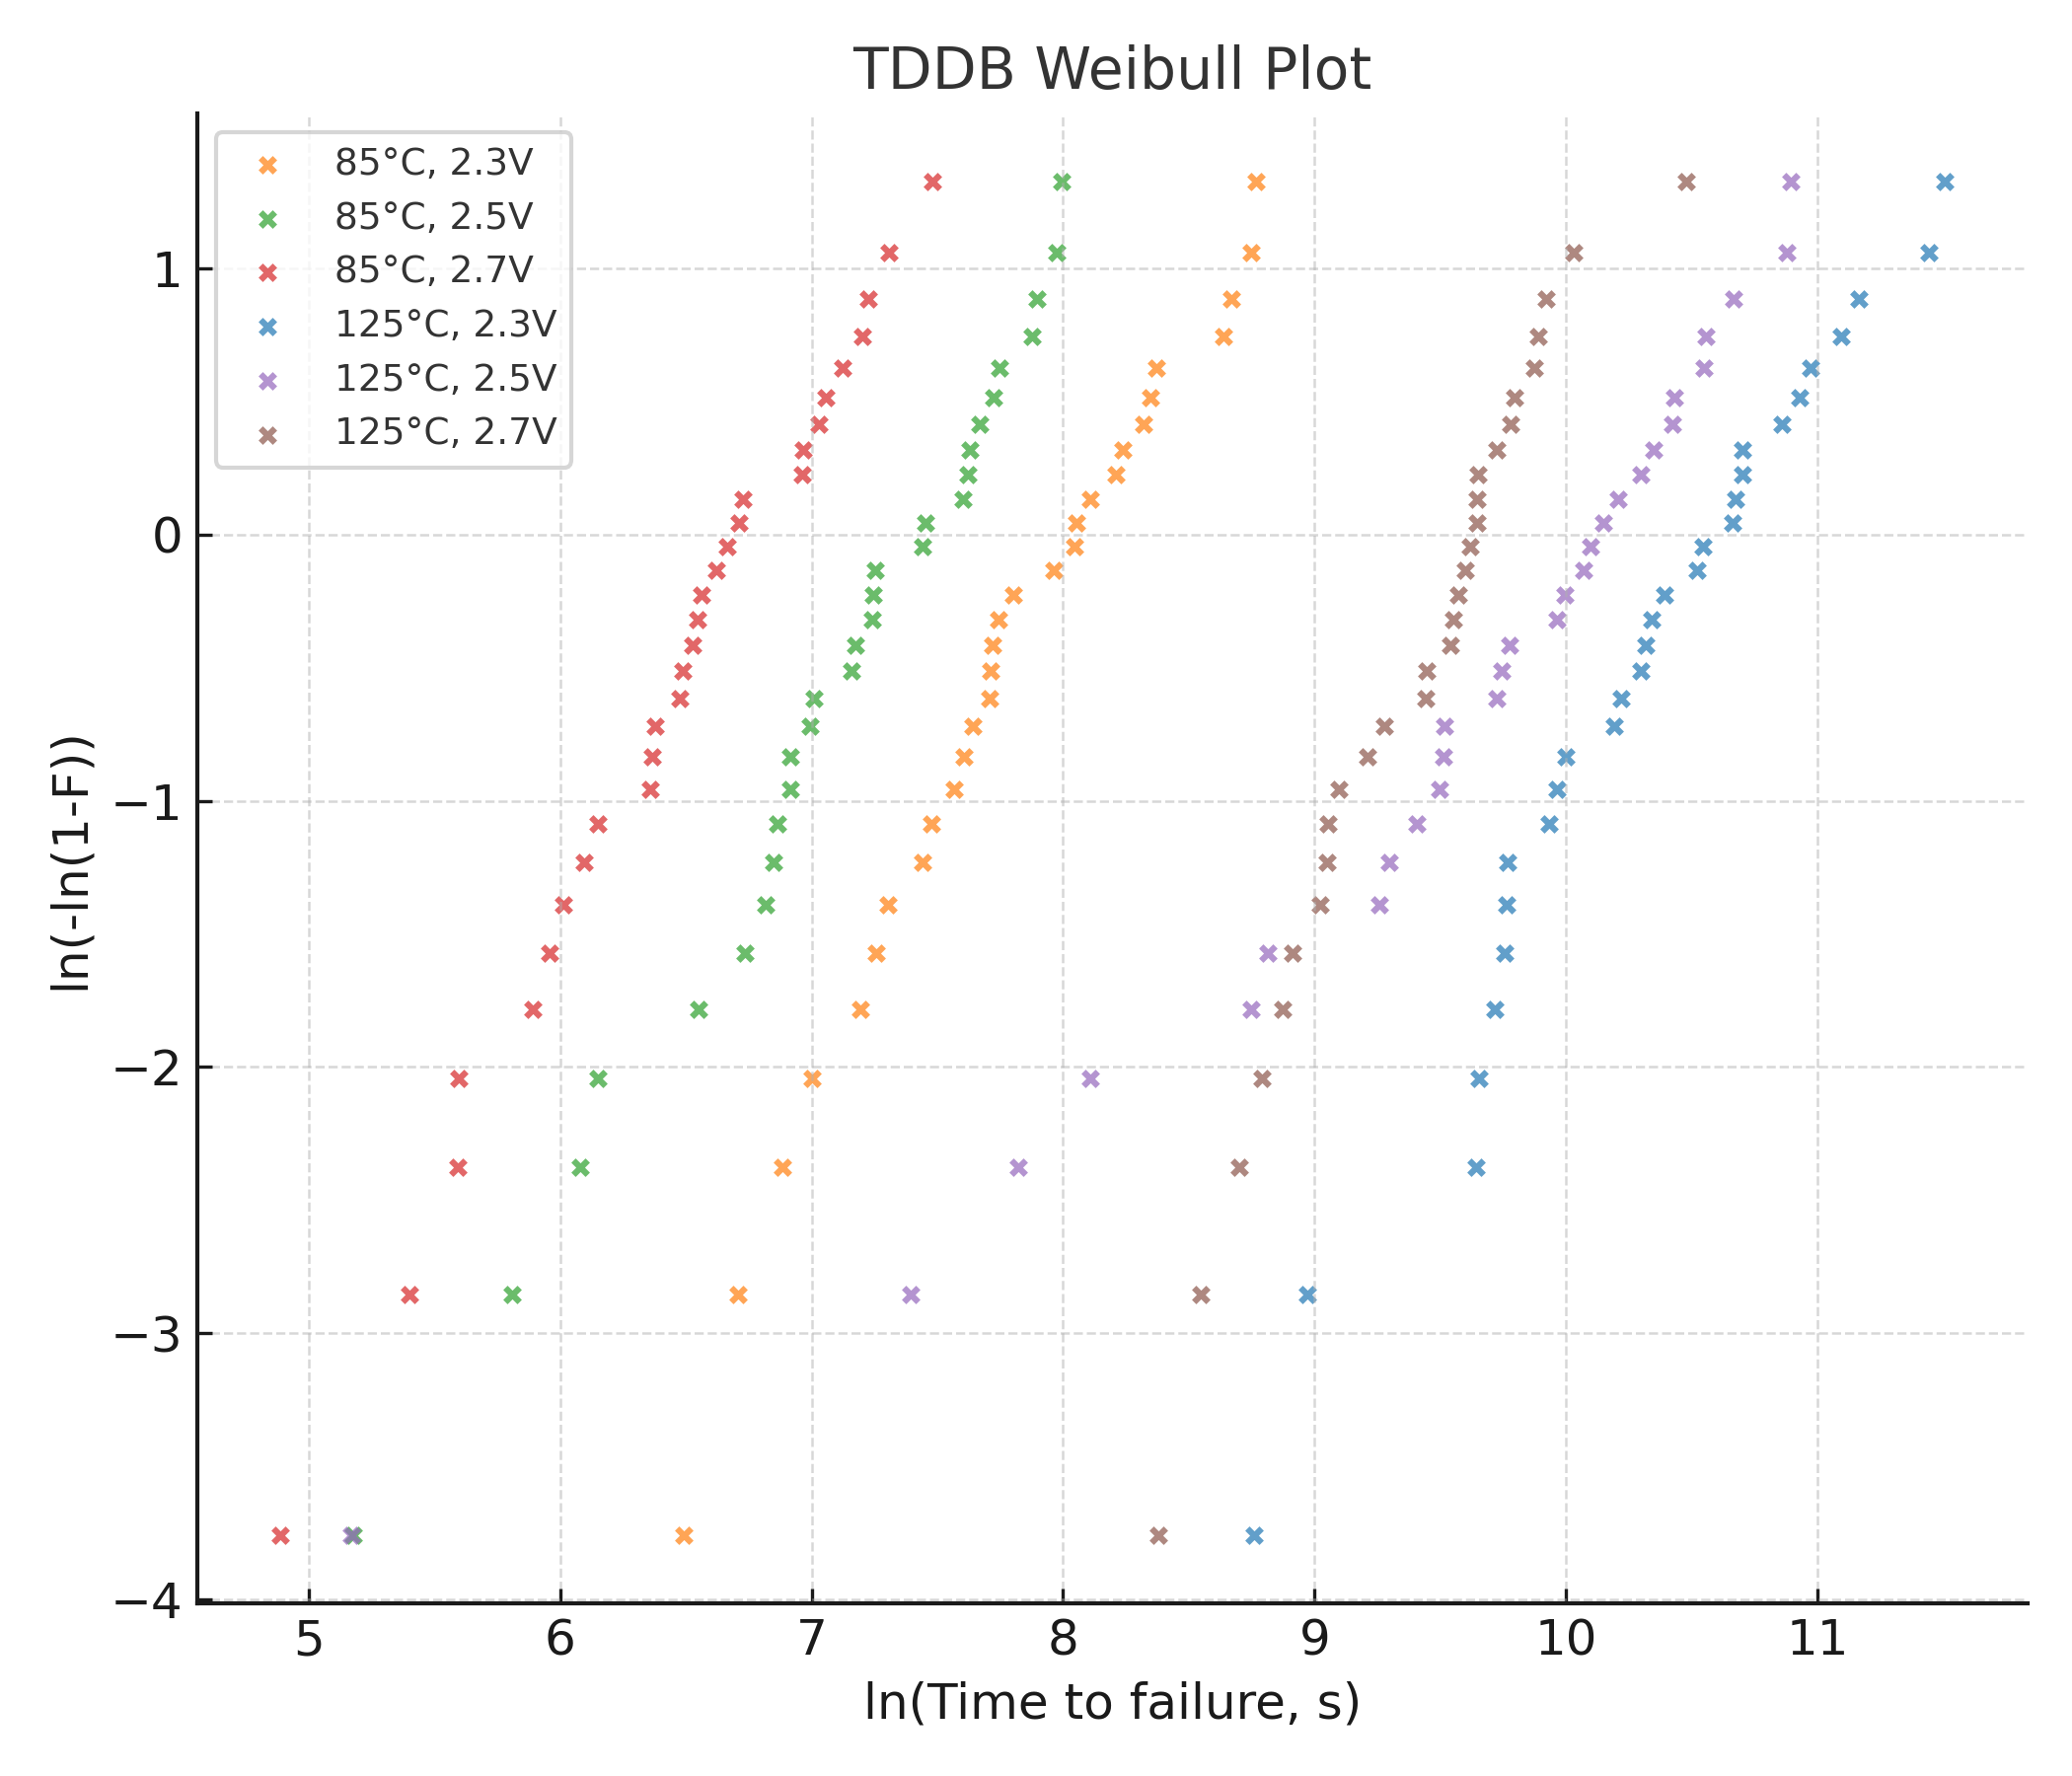
\includegraphics[width=\figw]{figures/fig4_tddb_weibull.png}
  \caption{TDDB Weibull plots with fitted slope $\beta \approx 1.3$ and scale $\eta$.}
  \label{fig:tddb_weibull}
\end{figure}

\subsection{Endurance}
\begin{figure}[!t]
  \centering
  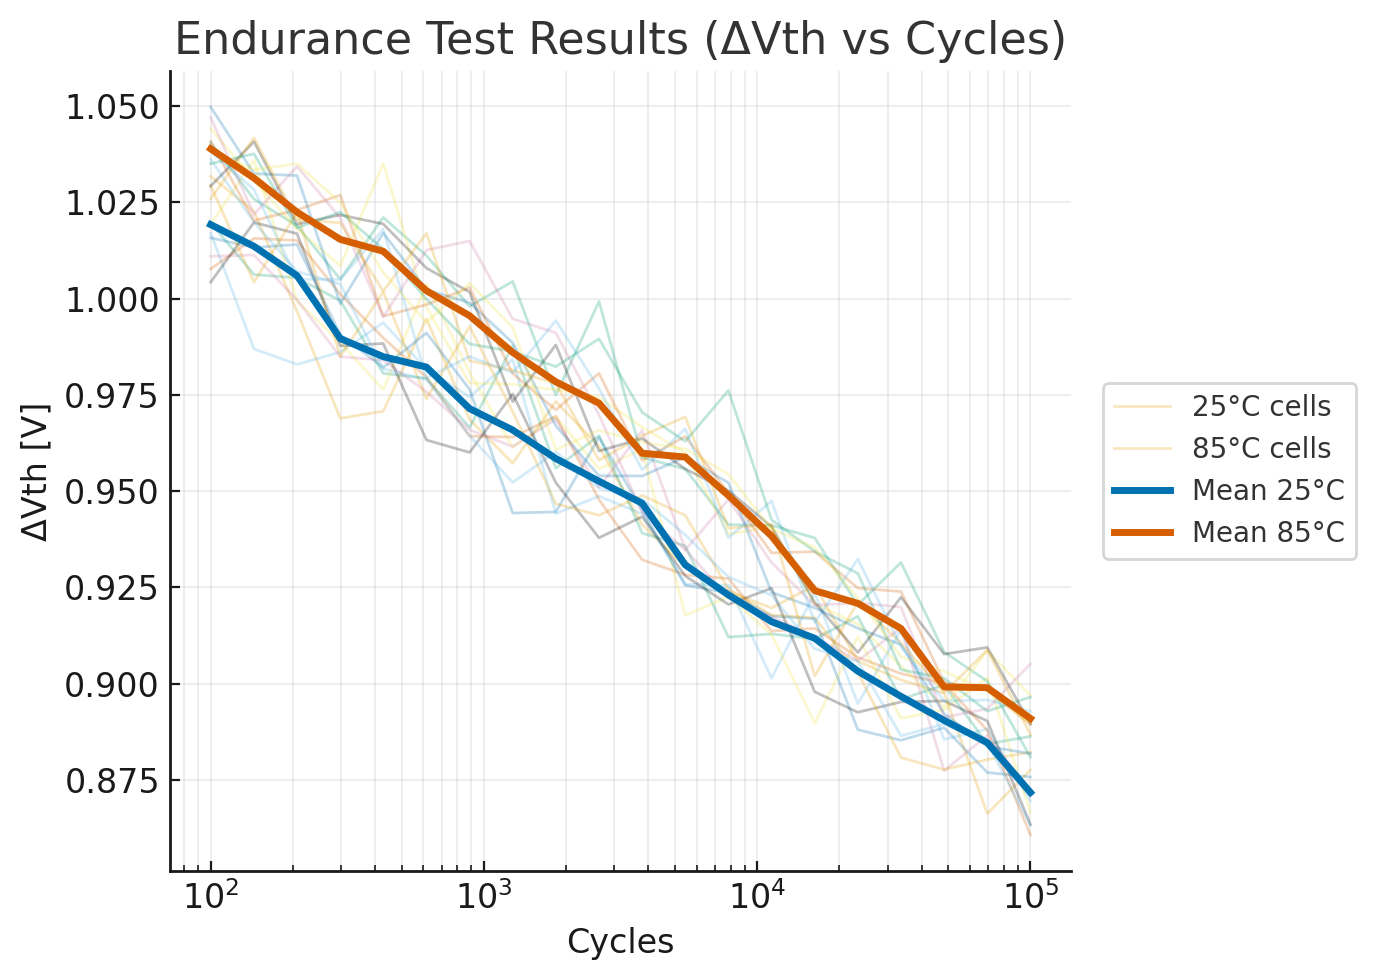
\includegraphics[width=\figw]{figures/fig5_endurance.png}
  \caption{Endurance characteristics ($\Delta V_{\mathrm{th}}$ vs. cycles). Up to $10^5$ cycles; window shrinks 20--30\%.}
  \label{fig:endurance}
\end{figure}

\subsection{Retention}
\begin{figure}[!t]
  \centering
  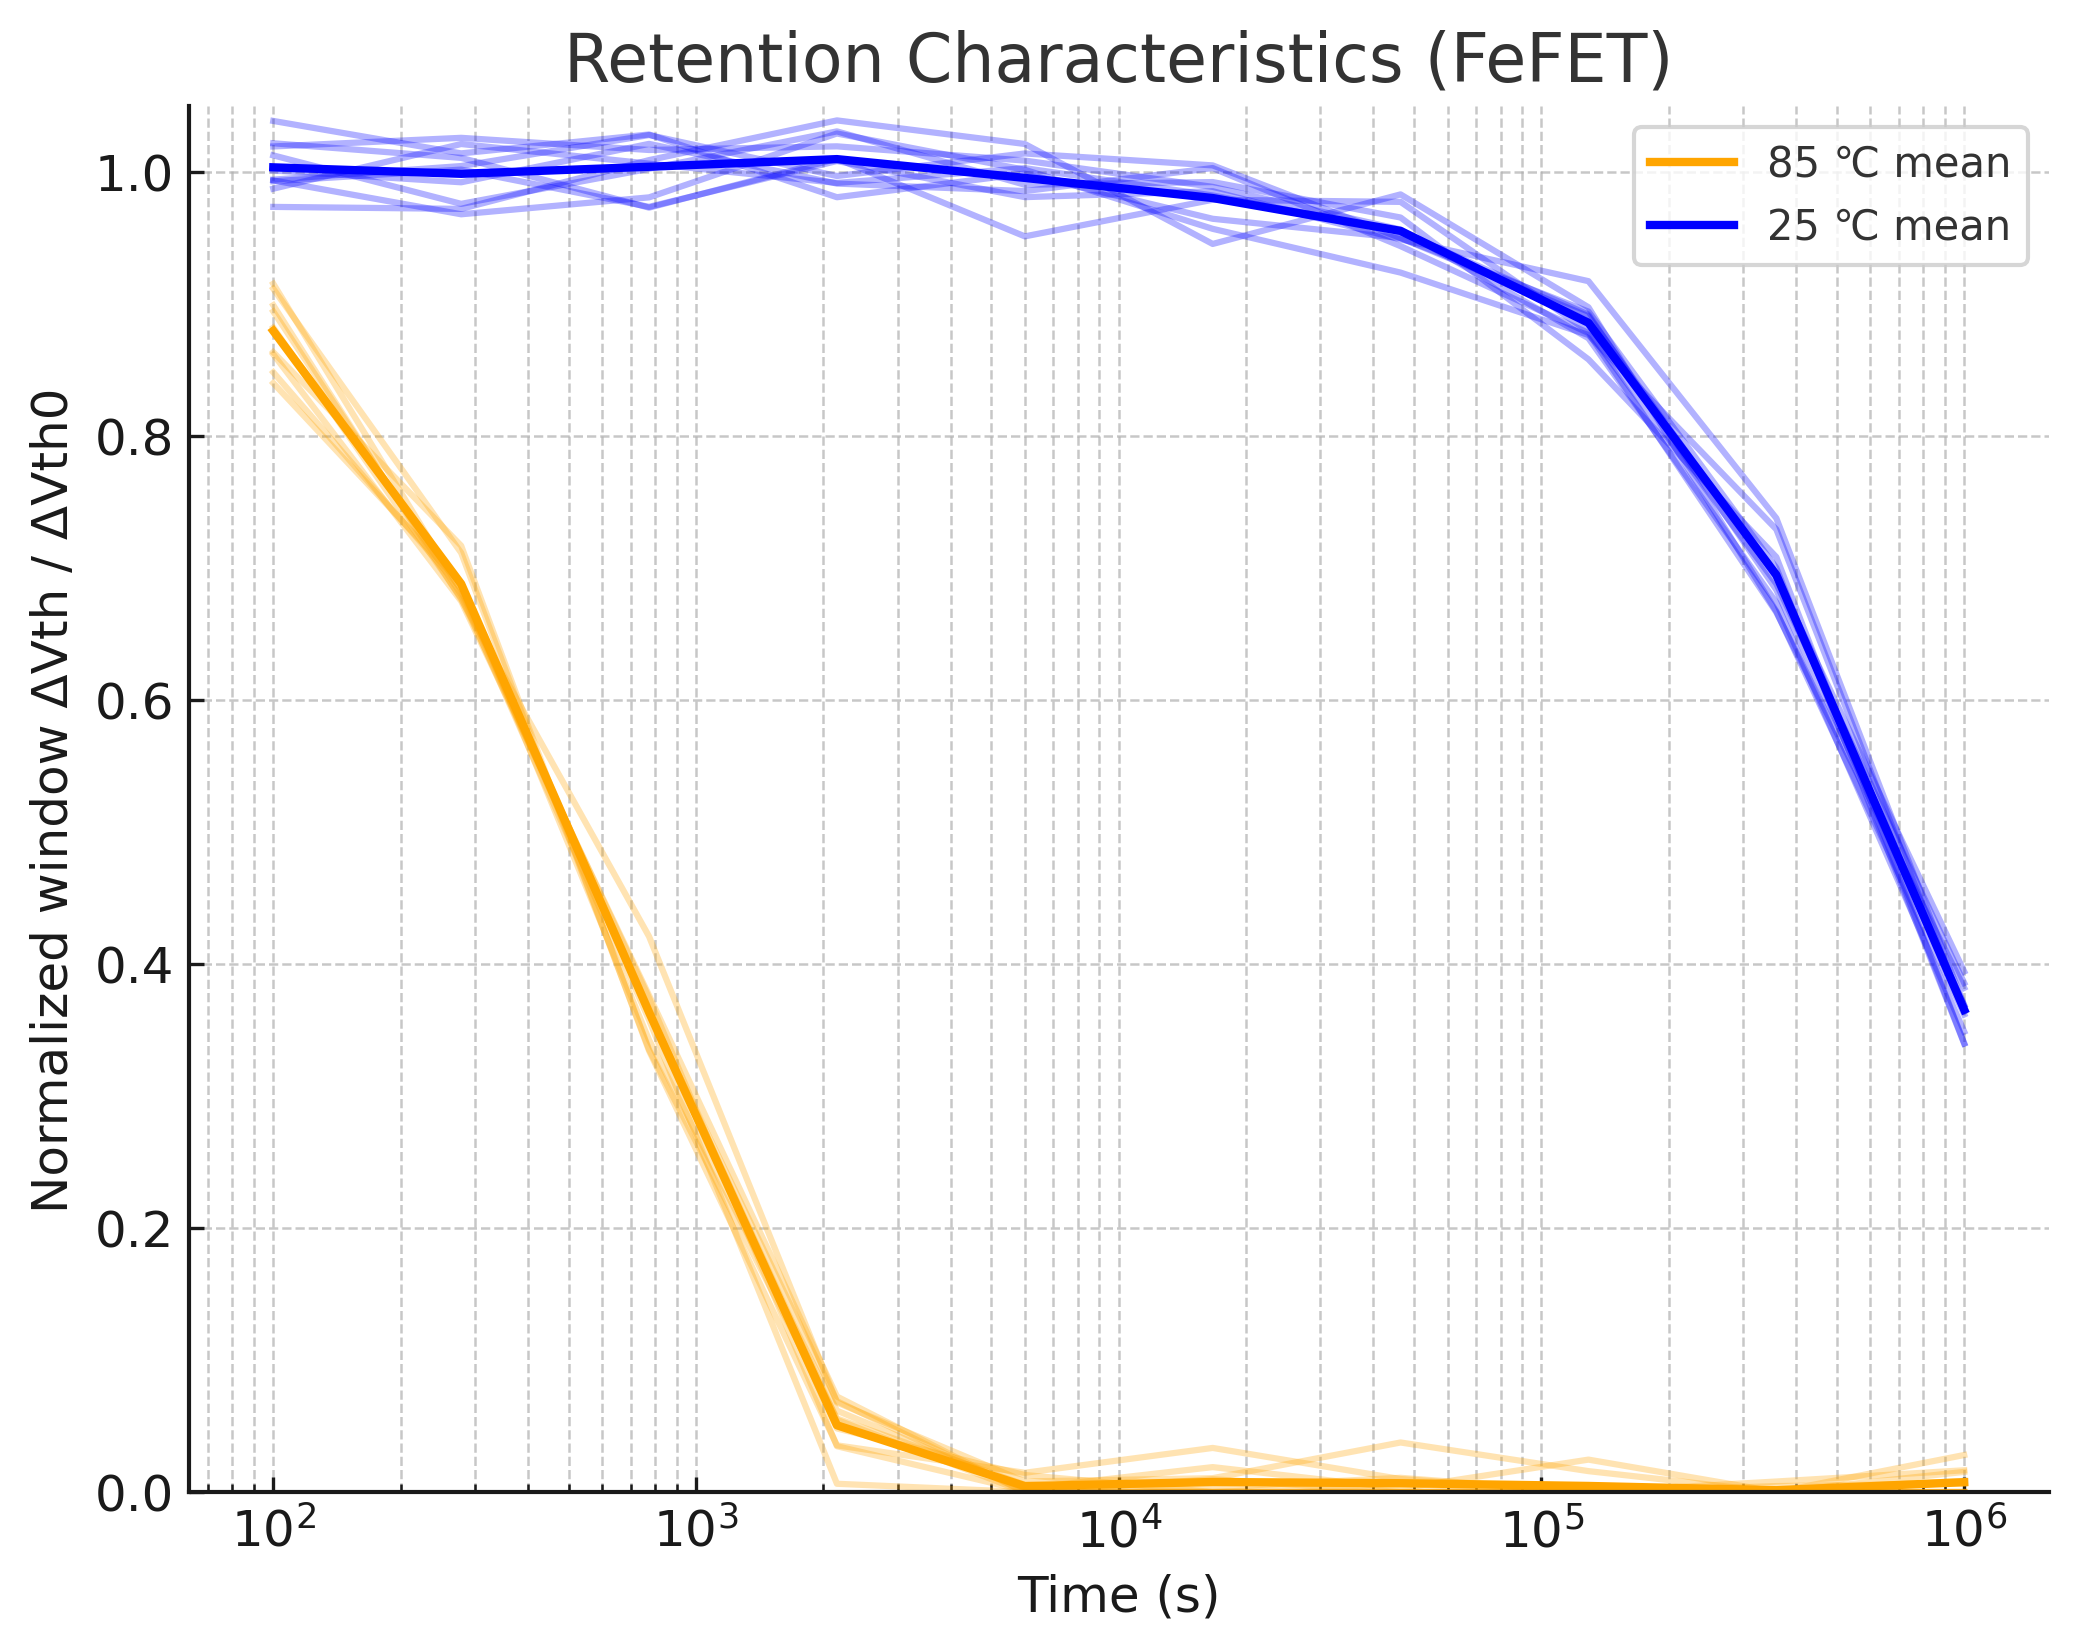
\includegraphics[width=\figw]{figures/fig6_retention.png}
  \caption{Retention summary (CDF and/or Arrhenius extrapolation).}
  \label{fig:retention}
\end{figure}

\subsection{Model Fits}
Time-to-failure under constant-voltage stress follows a Weibull law
\begin{equation}
  F(t)=1-\exp\!\left[-\left(\frac{t}{\etaW}\right)^{\betaW}\right],
\end{equation}
with slope $\betaW \approx 1.3$ and scale $\etaW$ extracted from Fig.~\ref{fig:tddb_weibull}.
Temperature acceleration is described by an Arrhenius relation
\begin{equation}
  \ln\!\left(\frac{t_2}{t_1}\right)=\frac{\Ea}{k}\!\left(\frac{1}{T_2}-\frac{1}{T_1}\right),
\end{equation}
yielding activation energies $\Ea \approx 0.78$~eV (2.3~V), $0.84$~eV (2.5~V), $0.88$~eV (2.7~V).
A compact endurance fit capturing memory-window shrink is
\begin{equation}
  \Delta \Vth(N) \approx 1.12 - 0.05\log_{10} N.
\end{equation}

% ========= System Architecture =========
\section{System Architecture (SRAM + FeFET)}
The SoC uses a single 1.8~V core domain for logic, SRAM, and FeFET access.
Write/erase pulses ($\pm$2.3--2.7~V, 1--50~$\mu$s) are generated by an on-chip charge pump.
A lightweight controller backs up SRAM contents to the FeFET array on power-fail detection and restores them at power-up.
An optional 3.3~V peripheral domain is kept for I/O and AMS (ADC/DAC, LDO).

% ---- page 3 top: Fig.8 (少し大きめだが左右いっぱいではない), Fig.9(1カラム)
\begin{figure*}[t]
  \centering
  \resizebox{0.80\textwidth}{!}{%
    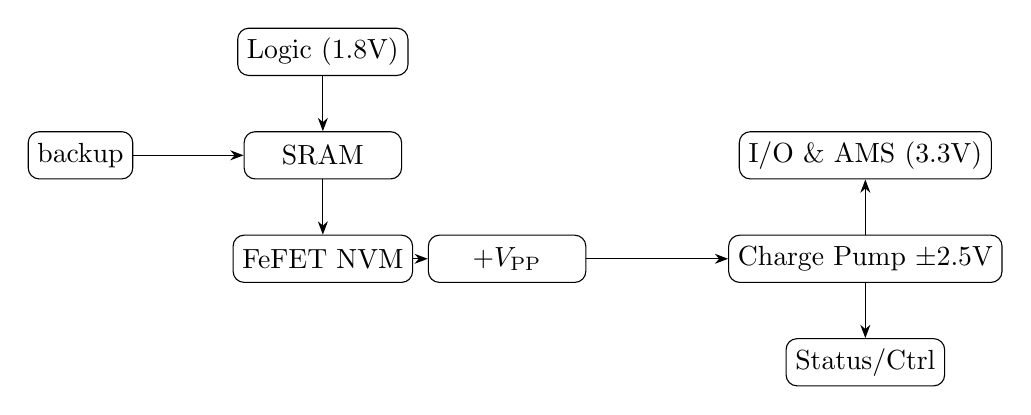
\begin{tikzpicture}[node distance=7mm, every node/.style={draw,rounded corners,minimum width=20mm,minimum height=6mm,align=center},>=Stealth,transform shape]
      \node (logic) {Logic (1.8V)};
      \node (sram) [below=of logic] {SRAM};
      \node (nvm)  [below=of sram] {FeFET NVM};
      \node (pump) [right=40mm of nvm] {Charge Pump $\pm$2.5V};
      \node (io)   [above=of pump] {I/O \& AMS (3.3V)};
      \node (stat) [below=of pump] {Status/Ctrl};
      \node (vpp)  [left=18mm of pump] {$+V_{\mathrm{PP}}$};
      \node (bk)   [left=14mm of sram, minimum width=13mm] {backup};
      \draw[->] (logic) -- (sram);
      \draw[->] (sram) -- (nvm);
      \draw[->] (nvm) -- (vpp);
      \draw[->] (vpp) -- (pump);
      \draw[->] (pump) -- (io);
      \draw[->] (pump) -- (stat);
      \draw[->] (bk.east) -- (sram.west);
    \end{tikzpicture}}
  \caption{System architecture with SRAM backup to FeFET.}
  \label{fig:system}
\end{figure*}

\begin{figure}[t]
  \centering
  \resizebox{0.85\columnwidth}{!}{%
  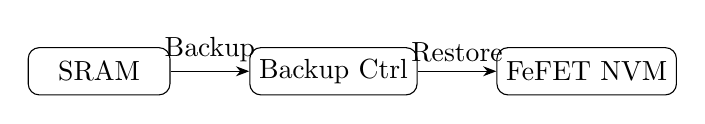
\begin{tikzpicture}[
      node distance=8mm,
      box/.style={draw,rounded corners,minimum width=18mm,minimum height=6mm}
  ]
    \node[box] (sram) {SRAM};
    \node[box, right=10mm of sram] (ctrl) {Backup Ctrl};
    \node[box, right=10mm of ctrl] (nvm)  {FeFET NVM};
    \draw[-{Stealth}] (sram) -- node[above]{Backup} (ctrl);
    \draw[-{Stealth}] (ctrl) -- node[above]{Restore} (nvm);
  \end{tikzpicture}}
  \caption{Backup/restore flow between SRAM and FeFET.}
  \label{fig:backup_flow}
\end{figure}

% ========= Discussion =========
\section{Discussion}
The HZO/Al$_2$O$_3$/TiN stack shows sufficient reliability for industrial/consumer embedded NVM.
For high-temperature automotive, improvements are required:
\begin{itemize}
  \item \textbf{Interlayer (IL) optimization}: Al$_2$O$_3$ thickness/composition tuning to mitigate wake-up/fatigue and reduce leakage.
  \item \textbf{Crystallinity control}: RTA window and TiN work-function engineering to stabilize ferroelectric phase and reduce variation.
  \item \textbf{Defect mitigation}: Precursor purity, ALD purge optimization, and post-deposition anneal to suppress oxygen-vacancy paths (helps TDDB/retention).
  \item \textbf{Circuit assists}: Verify-and-rewrite (background refresh at high-$T$), ECC, and adaptive write pulse shaping to slow window loss.
  \item \textbf{Array architecture}: Redundancy/repair and SRAM+FeFET hybrid usage to keep frequent writes on SRAM, reducing FeFET stress.
\end{itemize}

% ========= Conclusion =========
\section{Conclusion}
We realized a +1 mask FeFET module on 0.18~$\mu$m CMOS with only one additional ALD tool.
Devices exhibit $>10^5$ cycles and $>10$ years retention at 85$^\circ$C, verified by TZDB/TDDB/endurance/retention analyses.
The method extends mature-node lifetime and enables cost-effective embedded NVM for automotive/industrial/IoT.

% ========= Acknowledgment =========
\section*{Acknowledgment}
The author thanks collaborators for helpful discussions.

% ========= 参考文献(行間を微調整して詰める) =========
\begin{thebibliography}{1}\setlength{\itemsep}{0pt plus 0.3pt}
\bibitem{boscke2011} T. Böscke et al., \textit{Appl. Phys. Lett.}, vol. 99, p. 102903, 2011.
\bibitem{mueller2012} J. Müller et al., \textit{Appl. Phys. Lett.}, vol. 99, p. 112901, 2012.
\bibitem{mikolajick2019} T. Mikolajick et al., \textit{J. Appl. Phys.}, vol. 125, p. 204103, 2019.
\bibitem{mueller2015} J. Müller et al., \textit{IEEE Trans. Electron Devices}, vol. 62, no. 12, pp. 4158--4166, 2015.
\bibitem{park2020} J. Park et al., \textit{IEEE Electron Device Lett.}, vol. 41, no. 5, pp. 711--714, 2020.
\bibitem{nakamura2003} H. Nakamura et al., \textit{IEEE Trans. Device Mater. Rel.}, vol. 3, no. 4, pp. 132--136, 2003.
\bibitem{yamazaki2018} K. Yamazaki et al., \textit{Jpn. J. Appl. Phys.}, vol. 57, 04FB07, 2018.
\end{thebibliography}

% ========= Biography(小さめにして復活) =========
\section*{Biography}
\small
Shinichi Samizo has over 25 years of experience in semiconductor process integration and actuator development. After studying control theory and EM modeling in academia, he joined Seiko Epson in 1997 and worked on 0.35--0.18~$\mu$m CMOS logic/memory/HV integration, DRAM, and LCD drivers. Later he contributed to PZT actuator development and the PrecisionCore inkjet head. He is currently an independent researcher, publishing educational materials via the ``Project Design Hub''.

\end{document}
